\documentclass[11pt, oneside]{book}

% --- PACKAGES ---
\usepackage[a4paper, top=2.5cm, bottom=2.5cm, left=3cm, right=2.5cm]{geometry}
\usepackage{amsmath, amssymb, amsthm}
\usepackage{fontenc}
\usepackage{inputenc}
% microtype disabled for compatibility
\usepackage{xcolor}
\usepackage{graphicx}
\usepackage{booktabs}
\usepackage{longtable}
\usepackage{array}
\usepackage{enumitem}
\usepackage{listings}
\usepackage{fancyhdr}
\usepackage{titlesec}
\usepackage{tocloft}
\usepackage{hyperref}
\usepackage{mdframed}
\usepackage{tikz}
\usepackage{pgfplots}
\pgfplotsset{compat=1.18}
\usepackage{float}
\usepackage{caption}
\usepackage{subcaption}
\usepackage{setspace}
\usepackage{parskip}

% --- COLORS ---
\definecolor{quantblue}{RGB}{10, 40, 80}
\definecolor{quantgold}{RGB}{180, 140, 30}
\definecolor{lightgray}{RGB}{245, 245, 245}
\definecolor{codegray}{RGB}{240, 240, 245}
\definecolor{warnorange}{RGB}{200, 80, 20}
\definecolor{darkgreen}{RGB}{20, 100, 40}
\definecolor{steelblue}{RGB}{50, 100, 160}

% --- HYPERREF ---
\hypersetup{
    colorlinks=true,
    linkcolor=quantblue,
    urlcolor=steelblue,
    citecolor=quantgold,
    pdftitle={Institutional Quantitative Research Infrastructure: M/G/Infinity Portfolio Allocation System},
    pdfauthor={Quantitative Research Division}
}

% --- LISTINGS (CODE) ---
\lstdefinestyle{pythonstyle}{
    backgroundcolor=\color{codegray},
    commentstyle=\color{darkgreen}\itshape,
    keywordstyle=\color{quantblue}\bfseries,
    numberstyle=\tiny\color{gray},
    stringstyle=\color{warnorange},
    basicstyle=\ttfamily\footnotesize,
    breakatwhitespace=false,
    breaklines=true,
    captionpos=b,
    keepspaces=true,
    numbers=left,
    numbersep=5pt,
    showspaces=false,
    showstringspaces=false,
    showtabs=false,
    tabsize=4,
    language=Python,
    frame=single,
    rulecolor=\color{quantblue!30},
    xleftmargin=10pt,
    xrightmargin=5pt
}
\lstdefinestyle{sqlstyle}{
    backgroundcolor=\color{codegray},
    commentstyle=\color{darkgreen}\itshape,
    keywordstyle=\color{quantblue}\bfseries,
    stringstyle=\color{warnorange},
    basicstyle=\ttfamily\footnotesize,
    breaklines=true,
    captionpos=b,
    numbers=left,
    numberstyle=\tiny\color{gray},
    numbersep=5pt,
    frame=single,
    rulecolor=\color{quantblue!30},
    language=SQL,
    xleftmargin=10pt,
    morekeywords={CREATE, TABLE, VARCHAR, NUMERIC, BIGINT, BOOLEAN, DATE, PRIMARY, KEY, FOREIGN, REFERENCES, INDEX, ON, INSERT, INTO, SELECT, FROM, WHERE, AND, OR, JOIN, LEFT, INNER, GROUP, BY, ORDER, HAVING}
}

% --- CUSTOM ENVIRONMENTS ---
\newmdenv[
    backgroundcolor=quantblue!5,
    linecolor=quantblue,
    linewidth=2pt,
    leftmargin=0pt,
    rightmargin=0pt,
    innertopmargin=10pt,
    innerbottommargin=10pt,
    innerleftmargin=12pt,
    innerrightmargin=12pt
]{institutionbox}

\newmdenv[
    backgroundcolor=warnorange!8,
    linecolor=warnorange,
    linewidth=2pt,
    leftmargin=0pt,
    rightmargin=0pt,
    innertopmargin=10pt,
    innerbottommargin=10pt,
    innerleftmargin=12pt,
    innerrightmargin=12pt
]{warningbox}

\newmdenv[
    backgroundcolor=darkgreen!6,
    linecolor=darkgreen,
    linewidth=2pt,
    leftmargin=0pt,
    rightmargin=0pt,
    innertopmargin=10pt,
    innerbottommargin=10pt,
    innerleftmargin=12pt,
    innerrightmargin=12pt
]{successbox}

% --- SECTION FORMATTING ---
\titleformat{\chapter}[display]
    {\normalfont\huge\bfseries\color{quantblue}}
    {\chaptertitlename\ \thechapter}{20pt}{\Huge}
\titleformat{\section}
    {\normalfont\Large\bfseries\color{quantblue}}
    {\thesection}{1em}{}
\titleformat{\subsection}
    {\normalfont\large\bfseries\color{quantblue!80}}
    {\thesubsection}{1em}{}
\titleformat{\subsubsection}
    {\normalfont\normalsize\bfseries\color{quantblue!70}}
    {\thesubsubsection}{1em}{}

% --- HEADER/FOOTER ---
\pagestyle{fancy}
\fancyhf{}
\fancyhead[L]{\small\color{quantblue}\textit{Institutional Quant Infrastructure: M/G/$\infty$ Portfolio System}}
\fancyhead[R]{\small\color{quantblue}\thepage}
\fancyfoot[C]{\small\color{gray}\textit{Confidential Research Document}}
\renewcommand{\headrulewidth}{0.5pt}
\renewcommand{\headrule}{\hbox to\headwidth{\color{quantblue}\leaders\hrule height \headrulewidth\hfill}}

% --- MATH OPERATORS ---
\DeclareMathOperator{\Var}{Var}
\DeclareMathOperator{\E}{\mathbb{E}}

% --- TABLE OF CONTENTS ---
\setcounter{tocdepth}{2}
\renewcommand{\cftchapfont}{\bfseries\color{quantblue}}
\renewcommand{\cftsecfont}{\color{quantblue!80}}

\begin{document}

% ============================================================
%  TITLE PAGE
% ============================================================
\begin{titlepage}
    \pagecolor{quantblue}
    \color{white}
    \vspace*{2cm}
    \begin{center}
        {\Huge\bfseries Institutional Quantitative\\[0.3em]
        Research Infrastructure}\\[1.5em]
        {\rule{0.8\textwidth}{1pt}}\\[1.5em]
        {\Large\bfseries\color{quantgold} M/G/$\infty$ Queue-Based Valuation\\[0.3em]
        Mean-Reversion Portfolio System}\\[1.5em]
        {\rule{0.8\textwidth}{0.5pt}}\\[2em]
        {\large A Complete Step-by-Step Guide to Building a\\
        Fixed-Universe Quantitative Database\\
        and Walk-Forward Optimization Engine\\
        for \$0}\\[3em]
        {\normalsize\color{white!80}
        Covering: Fixed-Universe Construction (Russell 3000, 2025) $\cdot$ Point-in-Time Fundamentals\\
        PostgreSQL Schema Design $\cdot$ Python Data Pipeline\\
        M/G/$\infty$ Parameter Extraction $\cdot$ Walk-Forward Backtesting}\\[3em]
        {\small\color{quantgold}\textit{Note: Survivorship bias is intentionally not corrected in this version.\\
        The universe is fixed to the 2025 Russell 3000 constituent list.\\
        This is a mathematical research prototype, not a production trading system.}}\\[1em]
        {\rule{0.4\textwidth}{0.5pt}}\\[1em]
        {\normalsize Quantitative Research Division}\\[0.3em]
        {\small\color{white!70} Version 1.0 $\cdot$ 2025}
    \end{center}
    \vfill
    \begin{center}
        {\footnotesize\color{white!60}
        This document is intended for educational and research purposes only.\\
        Nothing herein constitutes investment advice.}
    \end{center}
\end{titlepage}
\pagecolor{white}
\color{black}

% ============================================================
%  PREFACE
% ============================================================
\chapter*{Preface}
\addcontentsline{toc}{chapter}{Preface}

This document is a complete technical blueprint for constructing an institutional-grade quantitative trading research environment from scratch, at zero cost. It bridges theoretical operations research---specifically, Erlang's M/G/$\infty$ queuing model---with the practical engineering required to deploy it against real market data.

\begin{institutionbox}
\textbf{The Core Thesis.} Portfolio capital allocation is mathematically equivalent to a service queue. Buy signals arrive randomly at some rate $\lambda_i$ per sector $i$; capital is deployed for a random holding duration with mean $\mu_i^{-1}$. The M/G/$\infty$ model provides a closed-form, provably optimal formula for how much capital to reserve in each sector bucket to keep stockout risk (running out of cash when signals arrive) equal across all sectors. The Square-Root Rule is the practical output of this model.
\end{institutionbox}

The pipeline described here spans four phases:
\begin{enumerate}[leftmargin=*, label=\textbf{Phase \arabic*.}]
    \item \textbf{Universe Construction} --- Download the current (2025) Russell 3000 constituent list from the iShares IWV ETF holdings file. This is a single CSV download. All tickers are fixed for the entire backtest.
    \item \textbf{Database Architecture} --- Design a PostgreSQL schema that is Point-in-Time (PiT) correct for fundamental data, with a fixed static universe.
    \item \textbf{Data Ingestion} --- Populate the database using the SEC EDGAR API for XBRL financial data and \texttt{yfinance} for prices, fetching from 2010 to present for every ticker in the fixed universe.
    \item \textbf{Strategy \& Validation} --- Extract M/G/$\infty$ parameters ($\lambda$, $\mu$) from the database and run Walk-Forward Optimization from 2010 to 2025.
\end{enumerate}

\begin{warningbox}
\textbf{Survivorship Bias Acknowledgement.} This version of the pipeline uses the \textit{current} Russell 3000 (as of 2025) as a fixed universe. Companies that were delisted, went bankrupt, or were acquired between 2010 and 2025 are \textbf{excluded}. This means the backtest will produce inflated returns relative to what a real strategy would have achieved---value traps and bankruptcies are missing from the signal set. This is a deliberate simplification: the goal of this document is to build and validate the M/G/$\infty$ allocation mathematics. Survivorship bias correction is left as a future extension once the core engine is verified.
\end{warningbox}

\tableofcontents

% ============================================================
%  PART I: THEORETICAL FOUNDATION
% ============================================================
\part{Theoretical Foundation}

\chapter{The M/G/$\infty$ Queue and the Square-Root Rule}

\section{Why Queuing Theory Belongs in Finance}

A portfolio manager running a valuation-based mean-reversion strategy faces a problem that is structurally identical to a service-operations problem. Consider the following analogy:

\begin{center}
\begin{tabular}{lll}
\toprule
\textbf{Service Operations} & & \textbf{Quant Portfolio} \\
\midrule
Delivery fleet (total capacity $C$) & $\Leftrightarrow$ & Total capital (\$500M) \\
Geographic regions & $\Leftrightarrow$ & Market sectors \\
Package arrival rate $\lambda_i$ & $\Leftrightarrow$ & Buy-signal rate per sector \\
Delivery duration $E[S_i]$ & $\Leftrightarrow$ & Avg.\ holding period to mean-reversion \\
Truck stockout (no truck available) & $\Leftrightarrow$ & Capital stockout (no cash to deploy) \\
\bottomrule
\end{tabular}
\end{center}

\vspace{0.5em}
In both cases, the system manager must pre-allocate capacity to regions/sectors such that (a) the probability of running out of capacity is equal across all regions/sectors, and (b) excess idle capacity is minimized.

\section{The M/G/$\infty$ Model}

\subsection{Model Specification}

The M/G/$\infty$ queue makes the following assumptions:

\begin{itemize}[leftmargin=*]
    \item \textbf{M (Markovian arrivals):} Buy signals arrive according to a Poisson process with rate $\lambda_i$ for sector $i$. This is the standard assumption for exogenous, unsynchronized event streams.
    \item \textbf{G (General service):} Holding periods follow an arbitrary distribution---we only require the mean $E[S_i] = \mu_i^{-1}$. This is critical: we do not assume normally distributed holding times. Mean-reversion can take 40 days or 400 days.
    \item \textbf{$\infty$ (Infinite servers):} Every arriving signal that has capital allocated to it is served immediately. There is no queue---only a capital stockout if the budget is exceeded.
\end{itemize}

\subsection{Steady-State Distribution}

Under these assumptions, the number of positions simultaneously open in sector $i$ at any time, denoted $N_i$, follows a Poisson distribution:

\begin{equation}
    N_i \sim \text{Poisson}(R_i), \quad \text{where} \quad R_i = \lambda_i \cdot E[S_i]
\end{equation}

$R_i$ is the \textit{offered load} of sector $i$---the expected number of open positions at any given moment. This is a direct consequence of Little's Law:
\begin{equation}
    L = \lambda W \implies R_i = \lambda_i \cdot \mu_i^{-1}
\end{equation}

\subsection{The Capital Buffer Problem}

Because $N_i \sim \text{Poisson}(R_i)$, the variance equals the mean:
\begin{equation}
    \Var(N_i) = R_i
\end{equation}

The portfolio manager sets a target service level: the probability that the number of simultaneous open positions exceeds the allocated capital slots $c_i$ should be at most $\alpha$ (e.g., $\alpha = 1\%$):
\begin{equation}
    P(N_i > c_i) \leq \alpha \quad \forall \, i
\end{equation}

\section{The Square-Root Allocation Rule}

\subsection{Derivation}

For large $R_i$, the Poisson distribution is well-approximated by a Normal distribution. Using the Normal approximation:
\begin{equation}
    P(N_i > c_i) = P\!\left(Z > \frac{c_i - R_i}{\sqrt{R_i}}\right) \leq \alpha
\end{equation}

where $Z \sim \mathcal{N}(0,1)$. Let $k = \Phi^{-1}(1 - \alpha)$ be the $z$-score for the target service level. Then:
\begin{equation}
    \frac{c_i - R_i}{\sqrt{R_i}} = k \implies \boxed{c_i = R_i + k\sqrt{R_i}}
\end{equation}

This is the \textbf{Square-Root Rule}. The key insight: $k$ is \textit{universal across all sectors}. The same $k$ gives the same stockout probability in every sector, regardless of how different the $\lambda_i$ and $\mu_i$ values are.

\subsection{Sector Budgeting}

Given total capital $C$ (in normalized units), the universal $k$ is determined by the constraint:
\begin{equation}
    \sum_{i=1}^{5} c_i = C \implies \sum_{i=1}^{5} \left(R_i + k\sqrt{R_i}\right) = C
\end{equation}

Solving for $k$:
\begin{equation}
    k = \frac{C - \sum_{i=1}^{5} R_i}{\sum_{i=1}^{5} \sqrt{R_i}}
\end{equation}

Once $k$ is determined, apply the Square-Root Rule to each sector to get the capital allocation $c_i$.

\subsection{Numerical Example}

Suppose the five sectors have the following calibrated parameters:

\begin{center}
\begin{tabular}{lcccc}
\toprule
\textbf{Sector} & $\lambda_i$ (signals/yr) & $E[S_i]$ (yrs) & $R_i$ & $\sqrt{R_i}$ \\
\midrule
Technology & 30 & 0.33 & 10.0 & 3.16 \\
Healthcare & 18 & 0.50 & 9.0 & 3.00 \\
Financials & 12 & 0.75 & 9.0 & 3.00 \\
Industrials & 8 & 0.60 & 4.8 & 2.19 \\
Consumer Goods & 10 & 0.40 & 4.0 & 2.00 \\
\midrule
\textbf{Total} & & & \textbf{36.8} & \textbf{13.35} \\
\bottomrule
\end{tabular}
\end{center}

With $C = 50$ capital units and $\alpha = 1\%$ (so $k$ is determined by the formula above):
\begin{equation}
    k = \frac{50 - 36.8}{13.35} = \frac{13.2}{13.35} \approx 0.989
\end{equation}

Capital allocations:
\begin{align*}
    c_{\text{Tech}} &= 10.0 + 0.989 \times 3.16 = 13.1 \text{ units} \\
    c_{\text{HC}} &= 9.0 + 0.989 \times 3.00 = 11.97 \text{ units} \\
    c_{\text{Fin}} &= 9.0 + 0.989 \times 3.00 = 11.97 \text{ units} \\
    c_{\text{Ind}} &= 4.8 + 0.989 \times 2.19 = 6.97 \text{ units} \\
    c_{\text{CG}} &= 4.0 + 0.989 \times 2.00 = 5.98 \text{ units} \\
    \textbf{Total} &= \mathbf{49.99} \approx 50 \checkmark
\end{align*}

\section{Why Valuation-Based Signals, Not Price}

Price-based signals (moving average crossovers, RSI) are stationary by construction---they have no economic foundation for mean-reversion. Valuation-based signals, by contrast, have a fundamental anchor:

\begin{institutionbox}
\textbf{The Graham Valuation Principle.} A stock's intrinsic value is determined by its earnings power and asset base, not its recent price trajectory. When a stock's P/E (or P/B, EV/EBITDA) falls more than 2 standard deviations below its own historical mean, there is a quantifiable margin of safety. The market is mispricing the asset relative to its fundamental generating capacity. Mean-reversion here is not a statistical artifact---it is an economic expectation.
\end{institutionbox}

The signal process: for stock $j$ in sector $i$ on date $t$,
\begin{equation}
    \text{Signal}_{j,t} = \mathbf{1}\!\left[\text{PE}_{j,t} < \overline{\text{PE}}_{j,\tau} - 2\sigma_{\text{PE},j,\tau}\right]
\end{equation}

where $\overline{\text{PE}}_{j,\tau}$ and $\sigma_{\text{PE},j,\tau}$ are the rolling mean and standard deviation of stock $j$'s P/E ratio over the trailing window $\tau$ (typically 5 years). The arrival rate $\lambda_i$ is then the count of such signals in sector $i$ per unit time.

% ============================================================
%  PART II: DATA INFRASTRUCTURE
% ============================================================
\part{Data Infrastructure}

\chapter{Universe Construction: Fixed Russell 3000 (2025)}

\section{Design Decision: Fixed Universe}

\begin{warningbox}
\textbf{Known Limitation.} The approach in this chapter introduces survivorship bias by design. The universe is fixed to companies that exist in the Russell 3000 as of June 2025. Companies that failed, were acquired, or were delisted between 2010 and 2025 are absent. For a mathematical prototype focused on validating the M/G/$\infty$ allocation engine, this is acceptable. It is not acceptable for production use.
\end{warningbox}

The universe source is the iShares IWV ETF holdings file (\texttt{IWV\_holdings25.csv}), downloaded directly from iShares (free, no account required). The file contains one row per holding with the following columns already populated for us:

\begin{center}
\begin{tabular}{lll}
\toprule
\textbf{CSV Column} & \textbf{Content} & \textbf{We Use It For} \\
\midrule
\texttt{Ticker}     & e.g.\ \texttt{MSFT}, \texttt{AAPL} & Primary key everywhere \\
\texttt{Name}       & e.g.\ \texttt{MICROSOFT CORP}       & \texttt{company\_name} in DB \\
\texttt{Sector}     & GICS Level 1 (11 sectors)           & Sector buckets for M/G/$\infty$ \\
\texttt{Asset Class}& \texttt{Equity}, \texttt{Futures}\ldots & Filter: keep \texttt{Equity} only \\
\texttt{Exchange}   & \texttt{NYSE}, \texttt{NASDAQ}\ldots & Metadata \\
\texttt{Weight (\%)}& ETF weight at snapshot date         & Optional: market-cap proxy \\
\bottomrule
\end{tabular}
\end{center}

Everything else we need---prices and fundamentals---comes from \texttt{yfinance} in later phases.

\section{Parsing \texttt{IWV\_holdings25.csv}}

The file has 9 metadata rows before the real header, and 6 non-equity rows (futures, cash, margin) plus 2 footer rows that must be stripped. After cleaning, we get \textbf{2,645 clean equity tickers}.

\begin{lstlisting}[style=pythonstyle, caption={Parsing IWV\_holdings25.csv into a Clean Universe DataFrame}]
import pandas as pd

def load_iwv_universe(filepath: str = "IWV_holdings25.csv") -> pd.DataFrame:
    """
    Parse the iShares IWV holdings CSV into a clean universe DataFrame.

    The file structure (verified against Jun 2025 download):
      Rows 0-8  : iShares metadata (fund name, date, totals)
      Row 9     : Column headers  (Ticker, Name, Sector, Asset Class, ...)
      Row 10+   : Holdings data
      Last 2    : NaN row + BlackRock legal disclaimer -- auto-dropped

    Returns a DataFrame with columns:
      ticker, company_name, sector, exchange
    """
    # skiprows=9 skips metadata; row 9 becomes the header
    df = pd.read_csv(filepath, skiprows=9, header=0)

    # --- Filter 1: Keep equity holdings only ---
    # Removes: Futures (ESU5, RTYU5), Cash, Cash Collateral, Money Market
    df = df[df["Asset Class"] == "Equity"].copy()

    # --- Filter 2: Keep only valid US equity tickers ---
    # Removes: "-" (unlisted warrants/CVRs like OMNIAB),
    #          "P5N994" (Petrocorp escrow - no market), NaN footer rows
    df = df[df["Ticker"].notna()]
    df = df[df["Ticker"].str.match(r'^[A-Z]{1,5}$', na=False)]

    # --- Rename to our DB column names ---
    universe = df[["Ticker", "Name", "Sector", "Exchange"]].copy()
    universe.columns = ["ticker", "company_name", "sector", "exchange"]
    universe = universe.drop_duplicates(subset="ticker").reset_index(drop=True)

    print(f"Universe loaded: {len(universe)} clean equity tickers")
    print(f"Sectors: {universe['sector'].nunique()} GICS sectors")
    return universe

UNIVERSE = load_iwv_universe("IWV_holdings25.csv")
# Output:
# Universe loaded: 2645 clean equity tickers
# Sectors: 11 GICS sectors
\end{lstlisting}

\begin{successbox}
\textbf{What You Get For Free From The CSV.} Unlike the original plan that required a yfinance enrichment pass to get sector and company name, the IWV CSV already provides \texttt{Ticker}, \texttt{Name}, \texttt{Sector}, and \texttt{Exchange} for all 2,645 tickers. You can load the entire metadata table in one shot from this file with no additional API calls.
\end{successbox}

\section{Fundamental Data Strategy: yfinance vs.\ SEC EDGAR}

\begin{warningbox}
\textbf{Honest Assessment of Fundamentals Complexity.} The original plan proposed fetching fundamentals from SEC EDGAR's XBRL API (true Point-in-Time correctness). This is the right long-term approach but is genuinely hard as a first project: you must resolve CIK numbers for all 2,645 tickers, handle missing XBRL tags, normalise different accounting taxonomies, and deal with amended filings. For a first build, \texttt{yfinance} quarterly financials are strongly recommended as a pragmatic starting point.
\end{warningbox}

\texttt{yfinance} exposes quarterly financial statements going back several years via three DataFrames per ticker:

\begin{center}
\begin{tabular}{lll}
\toprule
\textbf{yfinance attribute} & \textbf{What it contains} & \textbf{Key fields we extract} \\
\midrule
\texttt{.quarterly\_financials}    & Income statement (quarterly) & Net Income, Total Revenue, EPS \\
\texttt{.quarterly\_balance\_sheet} & Balance sheet (quarterly)    & Total Assets, Total Equity, Debt \\
\texttt{.quarterly\_cashflow}       & Cash flow statement          & Operating CF, CapEx, Free CF \\
\bottomrule
\end{tabular}
\end{center}

\textbf{The key limitation:} \texttt{yfinance} returns data \textit{as it exists today}, not as it was originally filed. It does not tag a \texttt{filing\_date}. This means fundamentals are not strictly PiT-correct---you are implicitly treating the period end date as the availability date. For a mean-reversion backtest where signals reset quarterly, this introduces a modest look-ahead bias (up to $\sim$60 days average filing lag). Accept this for version 1 and document it clearly.

\begin{institutionbox}
\textbf{PiT Rule (Relaxed, v1).} In this implementation, a fundamental value for period ending \texttt{period\_end\_date} is treated as available on that same date. In reality it becomes available 40--75 days later (the SEC filing deadline). Your WFO results will therefore be slightly optimistic. The fix---tagging with real \texttt{filing\_date}s from EDGAR---is a clean future upgrade without changing any other part of the system.
\end{institutionbox}



\chapter{PostgreSQL Database Schema}

\section{Architecture Overview}

Three tables are all we need for this version. The schema is deliberately minimal: every column in it is either (a) loaded directly from the IWV CSV, (b) fetched by \texttt{yfinance}, or (c) derived from those two sources. Nothing more.

\begin{center}
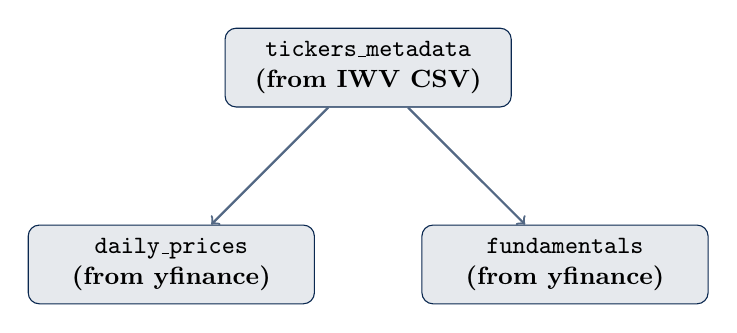
\begin{tikzpicture}[
    box/.style={rectangle, draw=quantblue, fill=quantblue!10, rounded corners, text width=3.4cm, text centered, minimum height=1cm, font=\small\bfseries},
    arr/.style={->, thick, color=quantblue!70}
]
    \node[box] (meta) at (2.5, 0)  {\texttt{tickers\_metadata}\\(from IWV CSV)};
    \node[box] (price) at (0, -2.5) {\texttt{daily\_prices}\\(from yfinance)};
    \node[box] (fund)  at (5, -2.5) {\texttt{fundamentals}\\(from yfinance)};

    \draw[arr] (meta) -- (price);
    \draw[arr] (meta) -- (fund);
\end{tikzpicture}
\end{center}

\textbf{What we dropped from the original schema and why:}
\begin{itemize}[leftmargin=*]
    \item \texttt{index\_constituents} / \texttt{static\_universe} --- redundant; \texttt{tickers\_metadata} \textit{is} the universe.
    \item \texttt{corporate\_actions} --- unnecessary because \texttt{yfinance} returns \texttt{adjusted\_close} already split- and dividend-adjusted. We never need to apply factors ourselves.
\end{itemize}

\section{Table Definitions}

\subsection{Table 1: \texttt{tickers\_metadata} --- The Master Roster}

Every column in this table comes directly from the IWV CSV. No API calls required to populate it.

\begin{lstlisting}[style=sqlstyle, caption={Master Roster Schema --- populated directly from IWV CSV}]
CREATE TABLE tickers_metadata (
    ticker          VARCHAR(12)  PRIMARY KEY,
    company_name    VARCHAR(255) NOT NULL,          -- CSV: "Name"
    sector          VARCHAR(64),                    -- CSV: "Sector" (GICS Level 1)
    exchange        VARCHAR(32),                    -- CSV: "Exchange"
    universe_type   VARCHAR(32)  NOT NULL DEFAULT 'FIXED_2025',
    snapshot_date   DATE         NOT NULL,          -- Jun 18, 2025 for this file
    created_at      TIMESTAMP    DEFAULT CURRENT_TIMESTAMP
);

CREATE INDEX idx_meta_sector ON tickers_metadata(sector);
\end{lstlisting}

\begin{successbox}
\textbf{No CIK column.} The original schema used CIK as the permanent identifier for joining XBRL data. Since we are fetching fundamentals via \texttt{yfinance} (which uses ticker symbols, not CIKs), we do not need a CIK column at all in v1. If you upgrade to EDGAR XBRL later, add a nullable \texttt{cik VARCHAR(12)} column at that time.
\end{successbox}


\subsection{Table 2: \texttt{daily\_prices} --- Price History}

End-of-day price data. The \texttt{adjusted\_close} column is the critical column for all calculations---it accounts for splits and dividends and is the only price series that correctly represents actual investor returns.

\begin{lstlisting}[style=sqlstyle, caption={Daily Prices Schema}]
CREATE TABLE daily_prices (
    price_id        BIGSERIAL    PRIMARY KEY,
    date            DATE         NOT NULL,
    ticker          VARCHAR(12)  REFERENCES tickers_metadata(ticker),
    open            NUMERIC(14,4),
    high            NUMERIC(14,4),
    low             NUMERIC(14,4),
    close           NUMERIC(14,4)  NOT NULL,
    adjusted_close  NUMERIC(14,4)  NOT NULL,  -- ALWAYS use this for calcs
    volume          BIGINT,
    UNIQUE (date, ticker)
);

CREATE INDEX idx_prices_ticker_date ON daily_prices(ticker, date);
CREATE INDEX idx_prices_date        ON daily_prices(date);
\end{lstlisting}

\begin{warningbox}
\textbf{Unadjusted Price Bias.} If a stock splits 2-for-1, its unadjusted price halves overnight. A naive algorithm sees a 50\% price drop and triggers a massive Buy signal. This is entirely spurious. Only \texttt{adjusted\_close}, which retroactively adjusts all historical prices for splits and dividends, produces economically meaningful return calculations. Never use raw \texttt{close} for strategy calculations.
\end{warningbox}

\subsection{Table 3: \texttt{fundamentals} --- Quarterly Financials}

Each row is one quarterly snapshot for one ticker, fetched from \texttt{yfinance}. The \texttt{period\_end\_date} is the fiscal quarter end. No \texttt{filing\_date} column---this is the v1 relaxed PiT approach discussed in Chapter 3.

\begin{lstlisting}[style=sqlstyle, caption={Simplified Fundamentals Schema (yfinance-sourced)}]
CREATE TABLE fundamentals (
    fundamental_id   BIGSERIAL   PRIMARY KEY,
    ticker           VARCHAR(12) REFERENCES tickers_metadata(ticker),
    period_end_date  DATE        NOT NULL,  -- Fiscal quarter end date

    -- Income Statement
    revenue          NUMERIC(18,2),
    gross_profit     NUMERIC(18,2),
    net_income       NUMERIC(18,2),
    eps_diluted      NUMERIC(12,4),

    -- Balance Sheet
    total_assets     NUMERIC(18,2),
    total_equity     NUMERIC(18,2),
    long_term_debt   NUMERIC(18,2),

    -- Cash Flow
    operating_cf     NUMERIC(18,2),   -- Operating cash flow
    capex            NUMERIC(18,2),

    -- Derived (compute on insert)
    book_value_per_share NUMERIC(12,4),  -- total_equity / shares_outstanding
    free_cash_flow   NUMERIC(18,2),      -- operating_cf - capex

    source           VARCHAR(16)  DEFAULT 'YFINANCE',
    created_at       TIMESTAMP    DEFAULT CURRENT_TIMESTAMP,

    UNIQUE (ticker, period_end_date)
);

CREATE INDEX idx_fund_ticker_date ON fundamentals(ticker, period_end_date);

-- Query Pattern: "Most recent fundamentals for AAPL as of 2018-01-15"
-- (relaxed PiT: treats period_end_date as availability date)
-- SELECT * FROM fundamentals
-- WHERE ticker = 'AAPL'
--   AND period_end_date <= '2018-01-15'
-- ORDER BY period_end_date DESC
-- LIMIT 1;
\end{lstlisting}

\chapter{Data Ingestion Pipeline}

\section{Phase 1: Universe Loading from IWV CSV}

One script, one source, one DB insert. The implementation lives in \texttt{src/ticker\_scraper.py}, and every column in \texttt{tickers\_metadata} comes directly from \texttt{IWV\_holdings25.csv}. The table itself is created by \texttt{sql/01\_tickers\_metadata.sql}; the loader only inserts rows.

\begin{lstlisting}[style=pythonstyle, caption={Loading IWV CSV Directly into PostgreSQL}]
from __future__ import annotations

from pathlib import Path

import psycopg2
from psycopg2.extras import execute_values
import pandas as pd

DEFAULT_CSV_PATH = Path(__file__).resolve().parent.parent / "IWV_holdings25.csv"
DEFAULT_DB_CONFIG = {
    "dbname": "quant_db",
    "user": "quant_user",
    "password": "your_password",
    "host": "localhost",
    "port": 5432,
}
DEFAULT_SNAPSHOT_DATE = "2025-06-18"


def load_iwv_universe(filepath: str | Path = DEFAULT_CSV_PATH) -> pd.DataFrame:
    """Parse IWV_holdings25.csv into a clean equity universe DataFrame."""
    df = pd.read_csv(filepath, skiprows=9, header=0)

    # Keep equity holdings only and drop non-standard tickers.
    df = df[df["Asset Class"] == "Equity"].copy()
    df = df[df["Ticker"].notna()]
    df = df[df["Ticker"].str.fullmatch(r'[A-Z]{1,5}', na=False)]

    universe = df[["Ticker", "Name", "Sector", "Exchange"]].copy()
    universe.columns = ["ticker", "company_name", "sector", "exchange"]
    universe = universe.drop_duplicates(subset="ticker").reset_index(drop=True)

    print(f"Universe loaded: {len(universe)} clean equity tickers")
    print(f"Sectors: {universe['sector'].nunique()} GICS sectors")
    return universe


def insert_universe_to_db(
    universe: pd.DataFrame,
    db_config: dict[str, object] = DEFAULT_DB_CONFIG,
    snapshot_date: str = DEFAULT_SNAPSHOT_DATE,
):
    """Insert the cleaned universe into an existing tickers_metadata table."""
    rows = [
        (row.ticker, row.company_name, row.sector, row.exchange, "FIXED_2025", snapshot_date)
        for row in universe.itertuples(index=False)
    ]

    conn = psycopg2.connect(**db_config)
    cur = conn.cursor()

    execute_values(cur, """
        INSERT INTO tickers_metadata
            (ticker, company_name, sector, exchange, universe_type, snapshot_date)
        VALUES %s
        ON CONFLICT (ticker) DO NOTHING
    """, rows)

    conn.commit()
    print(f"Inserted {len(rows)} tickers into tickers_metadata")
    cur.close()
    conn.close()

universe = load_iwv_universe()
insert_universe_to_db(universe)
# Output: Inserted 2645 tickers into tickers_metadata
\end{lstlisting}

\section{Phase 2: Price Data via yfinance}

\texttt{yfinance}'s \texttt{download()} function fetches adjusted daily closes for a list of tickers in batched requests. For 2,645 tickers fetching from 2010--01--01 to present, this takes roughly \textbf{30--90 minutes} depending on network speed. Run it once and never again.

\begin{lstlisting}[style=pythonstyle, caption={Bulk Price Download via yfinance (2010--Present)}]
import yfinance as yf
import psycopg2
from psycopg2.extras import execute_values
import pandas as pd
from datetime import date

def bulk_download_prices(tickers: list[str],
                         start: str = "2010-01-01",
                         batch_size: int = 100):
    """
    Download adjusted daily closes for all tickers, in batches of 100.
    yfinance handles batches internally but explicit batching gives
    cleaner error recovery if a batch fails.
    """
    conn = psycopg2.connect(
        dbname="quant_db", user="quant_user",
        password="your_password", host="localhost", port=5432
    )
    cur = conn.cursor()

    cur.execute("""
        CREATE TABLE IF NOT EXISTS daily_prices (
            date            DATE         NOT NULL,
            ticker          VARCHAR(12)  NOT NULL,
            adj_close       NUMERIC(14,4) NOT NULL,
            volume          BIGINT,
            PRIMARY KEY (date, ticker)
        )
    """)
    conn.commit()

    total_batches = (len(tickers) + batch_size - 1) // batch_size

    for i in range(0, len(tickers), batch_size):
        batch = tickers[i : i + batch_size]
        batch_num = i // batch_size + 1
        print(f"Batch {batch_num}/{total_batches}: {len(batch)} tickers")

        try:
            raw = yf.download(
                batch,
                start=start,
                end=str(date.today()),
                auto_adjust=True,   # Returns adjusted prices; 'Close' IS adj_close
                progress=False
            )
        except Exception as e:
            print(f"  ERROR on batch {batch_num}: {e}")
            continue

        # yfinance multi-ticker download has a MultiIndex:
        # columns = (metric, ticker)
        # We only need 'Close' (which is adjusted when auto_adjust=True)
        if isinstance(raw.columns, pd.MultiIndex):
            close_df = raw["Close"]   # shape: (dates, tickers)
            vol_df   = raw["Volume"]
        else:
            # Single ticker fallback
            close_df = raw[["Close"]].rename(columns={"Close": batch[0]})
            vol_df   = raw[["Volume"]].rename(columns={"Volume": batch[0]})

        rows = []
        for ticker in close_df.columns:
            series = close_df[ticker].dropna()
            vols   = vol_df[ticker] if ticker in vol_df.columns else None
            for dt, price in series.items():
                vol = int(vols[dt]) if vols is not None and dt in vols.index else None
                rows.append((dt.date(), ticker, float(price), vol))

        if rows:
            execute_values(cur, """
                INSERT INTO daily_prices (date, ticker, adj_close, volume)
                VALUES %s
                ON CONFLICT (date, ticker) DO NOTHING
            """, rows)
            conn.commit()
            print(f"  Inserted {len(rows):,} price rows")

    cur.close()
    conn.close()
    print("Price download complete.")

# Run it:
TICKERS = pd.read_sql(
    "SELECT ticker FROM tickers_metadata ORDER BY ticker",
    con=psycopg2.connect(dbname="quant_db", user="quant_user",
                         password="your_password", host="localhost")
)["ticker"].tolist()

bulk_download_prices(TICKERS, start="2010-01-01")
\end{lstlisting}

\begin{warningbox}
\textbf{Missing Price History for Young Companies.} Companies that IPO'd after 2010 will simply have shorter price history---\texttt{yfinance} returns whatever data exists. This is fine; the WFO engine will exclude a ticker from any window that starts before its IPO date (it will have no data for that period). No special handling required.
\end{warningbox}

\section{Phase 3: Fundamental Data via yfinance}

\texttt{yfinance} exposes quarterly financials via three per-ticker DataFrames. The challenge: unlike prices (where \texttt{download()} is batched), fundamentals must be fetched one ticker at a time. At $\sim$0.5--1 second per ticker, \textbf{2,645 tickers will take 45--90 minutes}. Run it overnight.

\begin{lstlisting}[style=pythonstyle, caption={Quarterly Fundamentals via yfinance (One Ticker at a Time)}]
import yfinance as yf
import psycopg2
from psycopg2.extras import execute_values
import pandas as pd
import time

def extract_yf_fundamentals(ticker: str) -> list[dict]:
    """
    Fetch quarterly income statement, balance sheet, and cash flow
    for one ticker from yfinance. Returns a list of dicts,
    one per quarter.
    """
    t = yf.Ticker(ticker)

    try:
        inc = t.quarterly_financials    # columns = quarter end dates
        bal = t.quarterly_balance_sheet
        cf  = t.quarterly_cashflow
    except Exception:
        return []

    if inc is None or inc.empty:
        return []

    records = []
    for period in inc.columns:  # Each column is a quarter-end date
        def safe_get(df, row):
            try:
                return float(df.loc[row, period]) if row in df.index else None
            except Exception:
                return None

        rec = {
            "ticker":          ticker,
            "period_end_date": period.date(),
            "revenue":         safe_get(inc, "Total Revenue"),
            "gross_profit":    safe_get(inc, "Gross Profit"),
            "net_income":      safe_get(inc, "Net Income"),
            "eps_diluted":     safe_get(inc, "Diluted EPS"),
            "total_assets":    safe_get(bal, "Total Assets"),
            "total_equity":    safe_get(bal, "Stockholders Equity"),
            "long_term_debt":  safe_get(bal, "Long Term Debt"),
            "operating_cf":    safe_get(cf,  "Operating Cash Flow"),
            "capex":           safe_get(cf,  "Capital Expenditure"),
        }
        # Derived fields
        rec["free_cash_flow"] = (
            (rec["operating_cf"] or 0) + (rec["capex"] or 0)
            # yfinance reports capex as negative, so adding gives FCF
        )
        records.append(rec)

    return records

def load_all_fundamentals(tickers: list[str]):
    conn = psycopg2.connect(
        dbname="quant_db", user="quant_user",
        password="your_password", host="localhost", port=5432
    )
    cur = conn.cursor()

    cur.execute("""
        CREATE TABLE IF NOT EXISTS fundamentals (
            fundamental_id  BIGSERIAL    PRIMARY KEY,
            ticker          VARCHAR(12)  REFERENCES tickers_metadata(ticker),
            period_end_date DATE         NOT NULL,
            revenue         NUMERIC(18,2),
            gross_profit    NUMERIC(18,2),
            net_income      NUMERIC(18,2),
            eps_diluted     NUMERIC(12,4),
            total_assets    NUMERIC(18,2),
            total_equity    NUMERIC(18,2),
            long_term_debt  NUMERIC(18,2),
            operating_cf    NUMERIC(18,2),
            capex           NUMERIC(18,2),
            free_cash_flow  NUMERIC(18,2),
            source          VARCHAR(16)  DEFAULT 'YFINANCE',
            created_at      TIMESTAMP    DEFAULT CURRENT_TIMESTAMP,
            UNIQUE (ticker, period_end_date)
        )
    """)
    conn.commit()

    failed = []
    for i, ticker in enumerate(tickers):
        if i % 100 == 0:
            print(f"Progress: {i}/{len(tickers)} ({i/len(tickers)*100:.1f}%)")

        records = extract_yf_fundamentals(ticker)
        if not records:
            failed.append(ticker)
            continue

        rows = [(
            r["ticker"], r["period_end_date"],
            r["revenue"], r["gross_profit"], r["net_income"], r["eps_diluted"],
            r["total_assets"], r["total_equity"], r["long_term_debt"],
            r["operating_cf"], r["capex"], r["free_cash_flow"]
        ) for r in records]

        execute_values(cur, """
            INSERT INTO fundamentals
                (ticker, period_end_date, revenue, gross_profit, net_income,
                 eps_diluted, total_assets, total_equity, long_term_debt,
                 operating_cf, capex, free_cash_flow)
            VALUES %s
            ON CONFLICT (ticker, period_end_date) DO NOTHING
        """, rows)
        conn.commit()
        time.sleep(0.3)  # Gentle on yfinance rate limits

    print(f"Done. Failed tickers ({len(failed)}): {failed[:20]}")
    cur.close()
    conn.close()

load_all_fundamentals(TICKERS)
\end{lstlisting}

\begin{warningbox}
\textbf{yfinance Fundamental Coverage.} yfinance typically returns 4--5 years of quarterly history per ticker (going back to around 2019--2020). It does \textbf{not} provide 15 years of quarterly fundamentals back to 2010 for most stocks. This means your WFO windows before $\sim$2019 will have no fundamental signal and cannot generate buy signals. In practice this means your effective backtest window with fundamentals is \textbf{2020--2025}, not 2010--2025. The price data still covers the full window, which is useful for benchmarking returns once a signal fires. If you need pre-2019 fundamentals you must switch to SEC EDGAR XBRL.
\end{warningbox}

% ============================================================
%  PART III: STRATEGY IMPLEMENTATION
% ============================================================
\part{Strategy Implementation}

\chapter{Extracting M/G/$\infty$ Parameters from the Database}

\section{The Valuation Signal}

With the database populated, parameter extraction follows a straightforward sequence. All queries use the three tables: \texttt{tickers\_metadata}, \texttt{daily\_prices}, and \texttt{fundamentals}.

\begin{warningbox}
\textbf{Relaxed PiT in These Queries.} Because fundamentals use \texttt{period\_end\_date} as the availability date (not a real \texttt{filing\_date}), the queries below filter on \texttt{period\_end\_date <= simulation\_date}. This is the v1 relaxation documented in Chapter 3.
\end{warningbox}

\subsection{Computing P/E Ratios at a Simulation Date}

\begin{lstlisting}[style=pythonstyle, caption={P/E Ratio Calculation (Relaxed PiT)}]
import pandas as pd
import numpy as np
import psycopg2

DB_CONFIG = {
    "dbname": "quant_db", "user": "quant_user",
    "password": "your_password", "host": "localhost", "port": 5432
}

def compute_pe(simulation_date: str) -> pd.DataFrame:
    """
    For each stock in the universe, compute P/E at simulation_date using:
      - Most recent adj_close on or before simulation_date
      - Most recent quarterly EPS with period_end_date <= simulation_date

    Returns DataFrame: ticker, sector, price, eps_diluted, pe_ratio
    """
    conn = psycopg2.connect(**DB_CONFIG)

    # Most recent price per ticker
    price_query = """
        SELECT DISTINCT ON (ticker)
            ticker, adj_close AS price
        FROM daily_prices
        WHERE date <= %(sim_date)s
        ORDER BY ticker, date DESC
    """

    # Most recent EPS per ticker (relaxed PiT: period_end_date as availability)
    eps_query = """
        SELECT DISTINCT ON (ticker)
            ticker, eps_diluted, period_end_date
        FROM fundamentals
        WHERE period_end_date <= %(sim_date)s
          AND eps_diluted IS NOT NULL
          AND eps_diluted > 0
        ORDER BY ticker, period_end_date DESC
    """

    prices = pd.read_sql(price_query, conn, params={"sim_date": simulation_date})
    eps    = pd.read_sql(eps_query,   conn, params={"sim_date": simulation_date})
    meta   = pd.read_sql("SELECT ticker, sector FROM tickers_metadata", conn)
    conn.close()

    df = meta.merge(prices, on="ticker", how="inner")
    df = df.merge(eps,    on="ticker", how="inner")
    df["pe_ratio"] = df["price"] / df["eps_diluted"]

    # Remove outliers (data quality gate)
    df = df[(df["pe_ratio"] > 1) & (df["pe_ratio"] < 200)]
    return df
\end{lstlisting}

\subsection{Generating Signals: The 2-SD Threshold}

\begin{lstlisting}[style=pythonstyle, caption={Rolling Valuation Signal Detection (Relaxed PiT)}]
def generate_signals(
    sim_date:      str,
    lookback_days: int = 504  # ~2 trading years (realistic with yfinance history)
) -> pd.DataFrame:
    """
    For each stock, check if P/E on sim_date is >=2 SD below its
    own rolling mean over the lookback window.
    Relaxed PiT: joins on period_end_date <= dp.date (not filing_date).
    """
    conn = psycopg2.connect(**DB_CONFIG)

    hist_query = """
        WITH daily_eps AS (
            SELECT
                dp.date,
                dp.ticker,
                dp.adj_close,
                f.eps_diluted
            FROM daily_prices dp
            CROSS JOIN LATERAL (
                SELECT eps_diluted
                FROM fundamentals
                WHERE ticker = dp.ticker
                  AND period_end_date <= dp.date
                  AND eps_diluted > 0
                ORDER BY period_end_date DESC
                LIMIT 1
            ) f
            WHERE dp.date BETWEEN %(start_date)s AND %(sim_date)s
        )
        SELECT
            de.date,
            de.ticker,
            tm.sector,
            de.adj_close / de.eps_diluted AS pe_ratio
        FROM daily_eps de
        JOIN tickers_metadata tm ON de.ticker = tm.ticker
        ORDER BY de.ticker, de.date
    """

    from datetime import datetime, timedelta
    start = (datetime.strptime(sim_date, '%Y-%m-%d')
             - timedelta(days=lookback_days * 1.5)).strftime('%Y-%m-%d')

    hist = pd.read_sql(
        hist_query, conn,
        params={'start_date': start, 'sim_date': sim_date}
    )
    conn.close()

    results = []
    for ticker, grp in hist.groupby('ticker'):
        grp = grp.sort_values('date').tail(lookback_days)
        if len(grp) < 126:  # Need at least 6 months of history
            continue

        rolling_mean = grp['pe_ratio'].mean()
        rolling_std  = grp['pe_ratio'].std()
        if rolling_std == 0:
            continue

        current_pe = grp.iloc[-1]['pe_ratio']
        z_score    = (current_pe - rolling_mean) / rolling_std
        results.append({
            'ticker':       ticker,
            'sector':       grp.iloc[-1]['sector'],
            'current_pe':   current_pe,
            'rolling_mean': rolling_mean,
            'rolling_std':  rolling_std,
            'z_score':      z_score,
            'is_signal':    z_score <= -2.0
        })

    df      = pd.DataFrame(results)
    signals = df[df['is_signal']].copy()
    print(f"Signals on {sim_date}: {len(signals)} across {signals['sector'].nunique()} sectors")
    return signals
\end{lstlisting}

\section{Computing $\lambda_i$ and $\mu_i$ from Historical Data}

To calibrate the M/G/$\infty$ queue, we need the signal arrival rate $\lambda_i$ and mean holding duration $\mu_i^{-1}$ for each sector $i$.

\begin{lstlisting}[style=pythonstyle, caption={M/G/Infinity Parameter Extraction}]
from scipy.stats import norm

def compute_mginfinity_params(
    train_start: str,
    train_end:   str,
    lookback_window_days: int = 1260
) -> dict:
    """
    Compute lambda_i and mu_i for each sector using training period data.

    lambda_i = number of 2-SD buy signals per year in sector i
    mu_i^{-1} = average days for P/E to revert to mean after signal

    Returns: {sector: {'lambda': float, 'mu_inv': float, 'R': float}}
    """
    import pandas as pd
    from datetime import datetime, timedelta

    train_start_dt = datetime.strptime(train_start, '%Y-%m-%d')
    train_end_dt   = datetime.strptime(train_end,   '%Y-%m-%d')
    years_in_sample = (train_end_dt - train_start_dt).days / 365.25

    # Step 1: Generate signals for every month in training period
    print("Generating historical signals for training period...")
    all_signals = []
    current = train_start_dt
    while current <= train_end_dt:
        sim_date = current.strftime('%Y-%m-%d')
        try:
            sigs = generate_signals(sim_date, lookback_days=lookback_window_days)
            sigs['signal_date'] = sim_date
            all_signals.append(sigs)
        except Exception as e:
            print(f"  Skipping {sim_date}: {e}")
        current += timedelta(days=21)  # Monthly sampling

    all_signals_df = pd.concat(all_signals, ignore_index=True)

    # Step 2: Compute lambda (signals per year per sector)
    signal_counts = (
        all_signals_df[all_signals_df['is_signal']]
        .groupby('sector')['ticker']
        .count()
    )
    lambda_i = (signal_counts / years_in_sample).to_dict()

    # Step 3: Compute mean holding duration (mu^{-1}) per sector
    # For each triggered signal, find how many days until P/E reverts above mean
    print("Computing mean reversion holding durations...")
    reversion_durations = {}
    conn = psycopg2.connect(**DB_CONFIG)

    triggered = all_signals_df[all_signals_df['is_signal']].copy()
    triggered = triggered.drop_duplicates(subset=['ticker', 'signal_date'])

    for _, row in triggered.iterrows():
        ticker      = row['ticker']
        sector      = row['sector']
        signal_date = row['signal_date']
        mean_pe     = row['rolling_mean']

        # Find first date after signal where P/E returns above rolling mean
        revert_query = """
            SELECT dp.date, dp.adj_close / f.eps_diluted AS pe_ratio
            FROM daily_prices dp
            CROSS JOIN LATERAL (
                SELECT eps_diluted FROM fundamentals
                WHERE ticker = dp.ticker
                  AND period_end_date <= dp.date
                  AND eps_diluted > 0
                ORDER BY period_end_date DESC LIMIT 1
            ) f
            WHERE dp.ticker = %(ticker)s
              AND dp.date > %(signal_date)s
              AND dp.date <= %(max_date)s
            ORDER BY dp.date
            LIMIT 500
        """
        max_date = (
            datetime.strptime(signal_date, '%Y-%m-%d') + timedelta(days=1500)
        ).strftime('%Y-%m-%d')

        try:
            future = pd.read_sql(
                revert_query, conn,
                params={'ticker': ticker, 'signal_date': signal_date,
                        'max_date': max_date}
            )

            reverted = future[future['pe_ratio'] >= mean_pe]
            if not reverted.empty:
                signal_dt  = datetime.strptime(signal_date, '%Y-%m-%d')
                revert_dt  = pd.to_datetime(reverted.iloc[0]['date'])
                duration_days = (revert_dt - signal_dt).days

                if sector not in reversion_durations:
                    reversion_durations[sector] = []
                reversion_durations[sector].append(duration_days)
        except Exception:
            pass

    conn.close()

    # mu^{-1} in years
    mu_inv_i = {
        sector: np.mean(durations) / 365.25
        for sector, durations in reversion_durations.items()
        if durations
    }

    # Combine into final parameter dict
    params = {}
    all_sectors = set(lambda_i.keys()) | set(mu_inv_i.keys())
    for sector in all_sectors:
        lam   = lambda_i.get(sector, 0)
        mu_inv = mu_inv_i.get(sector, 0.5)
        R = lam * mu_inv
        params[sector] = {
            'lambda':  lam,
            'mu_inv':  mu_inv,
            'R':       R,
            'sqrt_R':  np.sqrt(R) if R > 0 else 0
        }

    return params


def compute_capital_allocation(params: dict, total_capital: float) -> dict:
    """
    Apply the Square-Root Rule to compute sector capital allocations.

    c_i = R_i + k * sqrt(R_i)

    k is the universal buffer scalar solved by: sum(c_i) = total_capital
    """
    sum_R     = sum(p['R']      for p in params.values())
    sum_sqrtR = sum(p['sqrt_R'] for p in params.values())

    if sum_sqrtR == 0:
        raise ValueError("No valid sectors with positive R values")

    k = (total_capital - sum_R) / sum_sqrtR

    allocations = {}
    for sector, p in params.items():
        c_i = p['R'] + k * p['sqrt_R']
        allocations[sector] = {
            'R':          p['R'],
            'k':          k,
            'c_i':        max(c_i, 0),  # Cannot be negative
            'lambda':     p['lambda'],
            'mu_inv_yrs': p['mu_inv'],
        }

    print(f"\nUniversal buffer scalar k = {k:.4f}")
    print(f"{'Sector':<20} {'R_i':>8} {'c_i':>10} {'Capital%':>10}")
    print("-" * 52)
    for sector, alloc in allocations.items():
        pct = alloc['c_i'] / total_capital * 100
        print(f"{sector:<20} {alloc['R']:>8.2f} {alloc['c_i']:>10.2f} {pct:>9.1f}%")

    return allocations
\end{lstlisting}

\chapter{Walk-Forward Optimization}

\section{Methodology}

Walk-Forward Optimization (WFO) is the gold standard for validating quantitative trading strategies. Instead of optimizing on one historical period and testing on another, WFO continuously recalibrates the model as new data arrives, simulating the exact experience of a live portfolio manager.

\subsection{Window Configuration}

\begin{center}
\begin{tabular}{lll}
\toprule
\textbf{Parameter} & \textbf{Value} & \textbf{Rationale} \\
\midrule
Training window  & 2 years (504 trading days) & Matches yfinance fundamental history depth \\
Test (OOS) window & 1 year (252 trading days) & Annual recalibration \\
First training start & January 2020 & First year with reliable yfinance fundamentals \\
First test start & January 2022 & First OOS period \\
Final test end & December 2025 & 3-year OOS evaluation \\
\bottomrule
\end{tabular}
\end{center}

\begin{warningbox}
\textbf{Why the window starts in 2020, not 2010.} yfinance returns approximately 4--5 years of quarterly fundamentals per ticker. The P/E signal requires at least 6 months of EPS history before it can fire. A 2020 start is therefore the earliest realistic first training date. Price data from 2010 is still in the database and is used for return calculations once a position opens---it is not wasted.
\end{warningbox}

\begin{figure}[H]
\centering
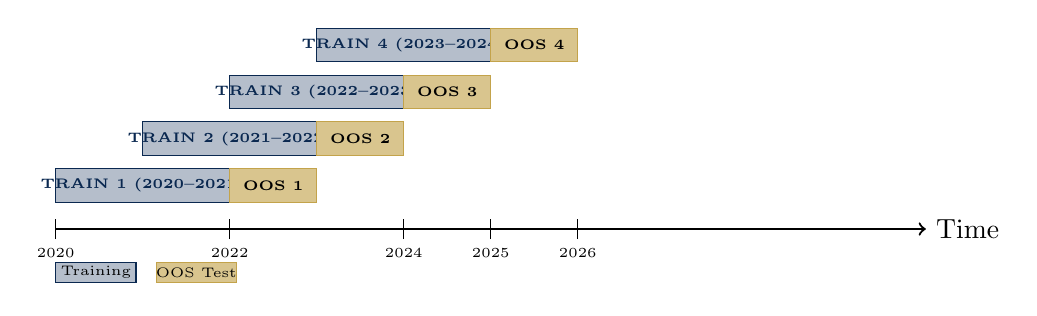
\begin{tikzpicture}[scale=0.85]
    % Timeline
    \draw[thick, ->] (0,0) -- (13,0) node[right] {Time};

    % Year markers
    \foreach \x/\yr in {0/2020, 2.6/2022, 5.2/2024, 6.5/2025, 7.8/2026} {
        \draw (\x, -0.15) -- (\x, 0.15);
        \node[below, font=\tiny] at (\x, -0.15) {\yr};
    }

    % Window 1: train 2020-2021, OOS 2022
    \draw[fill=quantblue!30, draw=quantblue] (0, 0.4) rectangle (2.6, 0.9)
        node[midway, font=\tiny\bfseries, color=quantblue] {TRAIN 1 (2020--2021)};
    \draw[fill=quantgold!50, draw=quantgold!80] (2.6, 0.4) rectangle (3.9, 0.9)
        node[midway, font=\tiny\bfseries] {OOS 1};

    % Window 2: train 2021-2022, OOS 2023
    \draw[fill=quantblue!30, draw=quantblue] (1.3, 1.1) rectangle (3.9, 1.6)
        node[midway, font=\tiny\bfseries, color=quantblue] {TRAIN 2 (2021--2022)};
    \draw[fill=quantgold!50, draw=quantgold!80] (3.9, 1.1) rectangle (5.2, 1.6)
        node[midway, font=\tiny\bfseries] {OOS 2};

    % Window 3: train 2022-2023, OOS 2024
    \draw[fill=quantblue!30, draw=quantblue] (2.6, 1.8) rectangle (5.2, 2.3)
        node[midway, font=\tiny\bfseries, color=quantblue] {TRAIN 3 (2022--2023)};
    \draw[fill=quantgold!50, draw=quantgold!80] (5.2, 1.8) rectangle (6.5, 2.3)
        node[midway, font=\tiny\bfseries] {OOS 3};

    % Window 4: train 2023-2024, OOS 2025
    \draw[fill=quantblue!30, draw=quantblue] (3.9, 2.5) rectangle (6.5, 3.0)
        node[midway, font=\tiny\bfseries, color=quantblue] {TRAIN 4 (2023--2024)};
    \draw[fill=quantgold!50, draw=quantgold!80] (6.5, 2.5) rectangle (7.8, 3.0)
        node[midway, font=\tiny\bfseries] {OOS 4};

    % Legend
    \draw[fill=quantblue!30, draw=quantblue] (0, -0.8) rectangle (1.2, -0.5)
        node[midway, font=\tiny] {Training};
    \draw[fill=quantgold!50, draw=quantgold!80] (1.5, -0.8) rectangle (2.7, -0.5)
        node[midway, font=\tiny] {OOS Test};
\end{tikzpicture}
\caption{Walk-Forward Optimization Window Structure (v1: 2-year train, 1-year OOS). Four OOS windows covering 2022--2025. Parameters are recalibrated annually.}
\end{figure}

\section{WFO Engine Implementation}

\begin{lstlisting}[style=pythonstyle, caption={Complete Walk-Forward Optimization Loop}]
from datetime import datetime, timedelta
import json

def run_walk_forward_optimization(
    total_capital_usd:   float = 500_000_000,
    train_years:         int   = 2,
    oos_years:           int   = 1,
    wfo_start:           str   = "2020-01-01",
    wfo_end:             str   = "2025-12-31",
    target_alpha:        float = 0.01  # 1% stockout probability target
) -> pd.DataFrame:
    """
    Main Walk-Forward Optimization loop.
    Returns DataFrame of annual OOS results.
    """

    from scipy.stats import norm
    k_target = norm.ppf(1 - target_alpha)

    results = []
    current_year = datetime.strptime(wfo_start, '%Y-%m-%d').year + train_years

    while True:
        # Define windows
        oos_start = f"{current_year}-01-01"
        oos_end   = f"{current_year}-12-31"
        train_start = f"{current_year - train_years}-01-01"
        train_end   = f"{current_year - 1}-12-31"

        if datetime.strptime(oos_end, '%Y-%m-%d') > datetime.strptime(wfo_end, '%Y-%m-%d'):
            break

        print(f"\n{'='*60}")
        print(f"TRAINING: {train_start} to {train_end}")
        print(f"OUT-OF-SAMPLE: {oos_start} to {oos_end}")
        print(f"{'='*60}")

        # --- TRAINING PHASE: Calibrate M/G/inf parameters ---
        try:
            params = compute_mginfinity_params(train_start, train_end)
            allocations = compute_capital_allocation(
                params,
                total_capital=100.0  # Use 100 units; scale to USD later
            )
        except Exception as e:
            print(f"  TRAINING FAILED: {e}")
            current_year += oos_years
            continue

        # --- OOS PHASE: Simulate portfolio from oos_start to oos_end ---
        oos_metrics = simulate_portfolio_oos(
            allocations      = allocations,
            oos_start        = oos_start,
            oos_end          = oos_end,
            total_capital    = total_capital_usd,
            target_alpha     = target_alpha
        )

        # Record results
        results.append({
            'train_start':         train_start,
            'train_end':           train_end,
            'oos_year':            current_year,
            'total_return_pct':    oos_metrics['total_return_pct'],
            'sharpe_ratio':        oos_metrics['sharpe_ratio'],
            'max_drawdown_pct':    oos_metrics['max_drawdown_pct'],
            'avg_stockout_pct':    oos_metrics['avg_stockout_pct'],
            'signals_triggered':   oos_metrics['signals_triggered'],
            'signals_rejected':    oos_metrics['signals_rejected'],
            'sector_imbalance':    oos_metrics['sector_stockout_std'],
            **{f"alloc_{s[:4]}": allocations.get(s, {}).get('c_i', 0)
               for s in allocations}
        })

        print(f"\n  OOS RESULT {current_year}:")
        print(f"    Return:       {oos_metrics['total_return_pct']:.2f}%")
        print(f"    Sharpe:       {oos_metrics['sharpe_ratio']:.3f}")
        print(f"    Max DD:       {oos_metrics['max_drawdown_pct']:.2f}%")
        print(f"    Stockout Rate:{oos_metrics['avg_stockout_pct']:.2f}%")

        current_year += oos_years

    results_df = pd.DataFrame(results)
    return results_df


def simulate_portfolio_oos(
    allocations:   dict,
    oos_start:     str,
    oos_end:       str,
    total_capital: float,
    target_alpha:  float
) -> dict:
    """
    Simulate the M/G/inf portfolio over the OOS period.
    On each day:
      1. Check for new buy signals (P/E drops 2-SD below mean)
      2. Accept signal if sector has available capital (c_i not exhausted)
      3. Reject signal if sector is fully deployed
      4. Close positions when P/E reverts to rolling mean
      5. Track PnL, drawdown, and stockout events

    Returns dict of performance metrics.
    """
    conn = psycopg2.connect(**DB_CONFIG)

    # Load trading days in OOS period
    trading_days = pd.read_sql(
        "SELECT DISTINCT date FROM daily_prices "
        "WHERE date BETWEEN %(s)s AND %(e)s ORDER BY date",
        conn, params={'s': oos_start, 'e': oos_end}
    )['date'].tolist()
    conn.close()

    # Portfolio state
    open_positions = {}    # {ticker: {entry_price, entry_date, sector, target_pe}}
    sector_deployed = {s: 0 for s in allocations}  # Units of capital deployed
    daily_pnl = []
    stockout_events = 0
    signals_triggered = 0
    signals_rejected  = 0

    # Normalize capital: 1 unit = total_capital / 100
    capital_unit = total_capital / 100.0

    for sim_date in trading_days:
        sim_date_str = sim_date.strftime('%Y-%m-%d')

        # Check for exits: close positions where P/E has reverted
        positions_to_close = []
        conn = psycopg2.connect(**DB_CONFIG)
        for ticker, pos in open_positions.items():
            cur_pe_df = pd.read_sql(
                """
                SELECT dp.adj_close / f.eps_diluted AS pe
                FROM daily_prices dp
                CROSS JOIN LATERAL (
                    SELECT eps_diluted FROM fundamentals
                    WHERE ticker=dp.ticker
                      AND period_end_date<=dp.date
                      AND eps_diluted > 0
                    ORDER BY period_end_date DESC LIMIT 1
                ) f
                WHERE dp.ticker=%(t)s AND dp.date=%(d)s
                """,
                conn, params={'t': ticker, 'd': sim_date_str}
            )
            if cur_pe_df.empty:
                continue

            current_pe = cur_pe_df.iloc[0]['pe']
            if current_pe >= pos['target_pe']:  # P/E reverted to mean
                # Calculate PnL
                cur_price_df = pd.read_sql(
                    "SELECT adj_close FROM daily_prices "
                    "WHERE ticker=%(t)s AND date=%(d)s",
                    conn, params={'t': ticker, 'd': sim_date_str}
                )
                if not cur_price_df.empty:
                    ret = (cur_price_df.iloc[0]['adj_close']
                           / pos['entry_price']) - 1
                    daily_pnl.append(ret * capital_unit)

                positions_to_close.append(ticker)
                sector_deployed[pos['sector']] -= 1

        for t in positions_to_close:
            del open_positions[t]

        # Check for new signals
        try:
            signals = generate_signals(sim_date_str)
        except Exception:
            conn.close()
            continue

        for _, sig in signals.iterrows():
            ticker = sig['ticker']
            sector = sig['sector']
            if ticker in open_positions:
                continue  # Already in position

            signals_triggered += 1

            # Check sector capacity (M/G/inf queue gate)
            max_slots = allocations.get(sector, {}).get('c_i', 0)
            deployed  = sector_deployed.get(sector, 0)

            if deployed >= max_slots:
                signals_rejected += 1  # STOCKOUT EVENT
                stockout_events  += 1
                continue

            # Open position
            entry_price_df = pd.read_sql(
                "SELECT adj_close FROM daily_prices "
                "WHERE ticker=%(t)s AND date=%(d)s",
                conn, params={'t': ticker, 'd': sim_date_str}
            )
            if entry_price_df.empty:
                continue

            open_positions[ticker] = {
                'entry_price': entry_price_df.iloc[0]['adj_close'],
                'entry_date':  sim_date_str,
                'sector':      sector,
                'target_pe':   sig['rolling_mean']
            }
            sector_deployed[sector] = sector_deployed.get(sector, 0) + 1

        conn.close()

    # Compute summary metrics
    if not daily_pnl:
        return {k: 0 for k in [
            'total_return_pct', 'sharpe_ratio', 'max_drawdown_pct',
            'avg_stockout_pct', 'signals_triggered', 'signals_rejected',
            'sector_stockout_std'
        ]}

    pnl_array   = np.array(daily_pnl)
    cum_returns = np.cumsum(pnl_array) / total_capital * 100
    total_ret   = cum_returns[-1] if len(cum_returns) > 0 else 0
    sharpe      = (np.mean(pnl_array) / (np.std(pnl_array) + 1e-10)) * np.sqrt(252)
    max_dd      = np.min(cum_returns - np.maximum.accumulate(cum_returns))
    stockout_pct = (stockout_events / max(signals_triggered, 1)) * 100

    return {
        'total_return_pct':   total_ret,
        'sharpe_ratio':       sharpe,
        'max_drawdown_pct':   max_dd,
        'avg_stockout_pct':   stockout_pct,
        'signals_triggered':  signals_triggered,
        'signals_rejected':   signals_rejected,
        'sector_stockout_std': np.std(list(sector_deployed.values()))
    }
\end{lstlisting}

\section{Interpreting Walk-Forward Results}

After running the full WFO loop, evaluate results against these institutional benchmarks:

\begin{center}
\begin{tabular}{llll}
\toprule
\textbf{Metric} & \textbf{Below Average} & \textbf{Acceptable} & \textbf{Institutional} \\
\midrule
Annual Return & $< 5\%$ & $5\%$--$12\%$ & $> 12\%$ \\
Sharpe Ratio & $< 0.5$ & $0.5$--$1.0$ & $> 1.0$ \\
Max Drawdown & $> -30\%$ & $-15\%$ to $-30\%$ & $< -15\%$ \\
Stockout Rate & $> 20\%$ & $5\%$--$20\%$ & $< 5\%$ \\
Sector Imbalance & High & Moderate & Near-zero \\
\bottomrule
\end{tabular}
\end{center}

The Stockout Rate is the M/G/$\infty$-specific diagnostic. If it exceeds your target $\alpha$ systematically, your $\lambda_i$ estimates were too low during calibration---the market generated more signals than the model anticipated. The Square-Root Rule's buffer $k\sqrt{R_i}$ was insufficient. Solutions: increase the training window, add a safety multiplier to $k$, or re-examine the signal definition.

\chapter{Regime Analysis and Stress Testing}

\section{Key Regimes in the WFO Window (2022--2025)}

The four OOS windows span two distinct macroeconomic regimes. This is a short window by institutional standards---one of the known limitations of a yfinance-only build. It is still sufficient to validate the M/G/$\infty$ allocation math.

\begin{center}
\begin{tabular}{p{2.2cm}p{3cm}p{3.5cm}p{3.5cm}}
\toprule
\textbf{Period} & \textbf{Regime} & \textbf{Expected Behaviour} & \textbf{M/G/$\infty$ Stress} \\
\midrule
2022 & Inflation + aggressive rate hikes & Growth stock collapse. Value signals fire heavily in Tech and Consumer. $\lambda$ elevated. & Tests if $k$ buffer is calibrated correctly when trained on 2020--2021. \\
2023 & Soft landing + AI boom & Rapid Tech re-rating. Short holding durations. High $\mu$, low $\mu^{-1}$. & Low stockout pressure. Tests if $R_i$ shrinks appropriately. \\
2024--2025 & Rate cuts + broad recovery & Moderate $\lambda$ across sectors. Strategy expected to perform steadily. & Baseline regime---results here most representative. \\
\bottomrule
\end{tabular}
\end{center}

\section{2020 Covid Crash: A Training Data Asset}

In this v1 build, 2020 falls inside the training window, not the OOS period. This is actually useful: the Covid crash is the most extreme $\lambda$ spike in recent history---every stock looked cheap simultaneously by P/E standards. Training on this event means the calibrated $k$ buffer will incorporate the experience of a systemic shock. The model will set a higher $k$ than if trained only on calm 2023--2024 data.

The diagnostic question for the 2022 OOS window is: \textit{did the model trained on 2020--2021 (including the crash and V-recovery) produce a $k$ buffer large enough to handle the more moderate but sustained $\lambda$ elevation of the inflation period?} If the stockout rate in 2022 is near the 1\% target, the training data inclusion was beneficial. If it is far above 1\%, the 2020 spike overfit $k$ in the wrong direction for a sustained-inflation regime.

% ============================================================
%  PART IV: APPENDICES
% ============================================================
\part{Appendices}

\chapter{Database Setup and Operations}

\section{PostgreSQL Installation and Configuration}

\begin{lstlisting}[style=pythonstyle, caption={Environment Setup Script}]
# Install PostgreSQL and Python dependencies
# Run in terminal:
# sudo apt-get install postgresql postgresql-contrib  (Linux)
# brew install postgresql  (macOS)

# Python dependencies
# pip install psycopg2-binary pandas numpy scipy yfinance requests

# Create the database
# sudo -u postgres psql
# CREATE DATABASE quant_db;
# CREATE USER quant_user WITH ENCRYPTED PASSWORD 'your_password';
# GRANT ALL PRIVILEGES ON DATABASE quant_db TO quant_user;

DB_CONFIG = {
    "dbname":   "quant_db",
    "user":     "quant_user",
    "password": "your_password",
    "host":     "localhost",
    "port":     5432
}

import psycopg2

def initialize_database():
    """Create all tables and indexes from scratch."""
    conn = psycopg2.connect(**DB_CONFIG)
    cur  = conn.cursor()

    # Read the SQL schema files and execute
    schema_files = [
        'sql/01_tickers_metadata.sql',
        'sql/02_daily_prices.sql',
        'sql/03_fundamentals.sql',
    ]
    for f in schema_files:
        with open(f) as fh:
            cur.execute(fh.read())
        conn.commit()
        print(f"Executed: {f}")

    cur.close()
    conn.close()
    print("Database initialized successfully.")
\end{lstlisting}

\section{Master Orchestration Script}

\begin{lstlisting}[style=pythonstyle, caption={Main Pipeline Runner}]
import logging
import pandas as pd
from datetime import datetime

logging.basicConfig(
    level=logging.INFO,
    format='%(asctime)s [%(levelname)s] %(message)s',
    handlers=[
        logging.FileHandler('quant_pipeline.log'),
        logging.StreamHandler()
    ]
)
logger = logging.getLogger(__name__)

def run_full_pipeline():
    """
    End-to-end data pipeline.
    Estimated total runtime on first run: ~2-3 hours.
      Phase 1: < 1 minute   (CSV load)
      Phase 2: 30-90 min    (price download, batched)
      Phase 3: 45-90 min    (fundamentals, one-by-one)
      Phase 4: < 5 min      (WFO on 4 windows)
    """
    start_time = datetime.now()
    logger.info("=== QUANT PIPELINE STARTED ===")

    # PHASE 1: Universe -- straight from IWV_holdings25.csv
    logger.info("Phase 1: Loading fixed universe from IWV_holdings25.csv")
    universe = load_iwv_universe("IWV_holdings25.csv")
    insert_universe_to_db(universe)
    tickers = universe["ticker"].tolist()
    logger.info(f"Phase 1 complete: {len(tickers):,} tickers loaded")

    # PHASE 2: Price data (2010-present) via yfinance, batched by 100
    logger.info("Phase 2: Downloading price data via yfinance (2010-present)")
    bulk_download_prices(tickers, start="2010-01-01", batch_size=100)
    logger.info("Phase 2 complete")

    # PHASE 3: Quarterly fundamentals via yfinance (one ticker at a time)
    logger.info("Phase 3: Downloading quarterly fundamentals via yfinance")
    logger.info("  NOTE: yfinance covers ~2019-present. Pre-2019 will be empty.")
    load_all_fundamentals(tickers)
    logger.info("Phase 3 complete")

    # PHASE 4: Walk-Forward Optimization (2020-2025, 2yr train, 1yr OOS)
    logger.info("Phase 4: Running Walk-Forward Optimization (2022-2025 OOS)")
    results = run_walk_forward_optimization(
        total_capital_usd = 500_000_000,
        train_years       = 2,
        oos_years         = 1,
        wfo_start         = "2020-01-01",
        wfo_end           = "2025-12-31",
        target_alpha      = 0.01
    )
    results.to_csv('wfo_results.csv', index=False)
    logger.info(f"Phase 4 complete. {len(results)} OOS windows. Saved to wfo_results.csv")

    elapsed = datetime.now() - start_time
    logger.info(f"=== PIPELINE COMPLETE in {elapsed} ===")

if __name__ == "__main__":
    run_full_pipeline()
\end{lstlisting}

\chapter{Data Quality Checklist}

Before running any WFO, verify your database passes these checks. All queries use the three actual table names: \texttt{tickers\_metadata}, \texttt{daily\_prices}, \texttt{fundamentals}.

\begin{enumerate}[leftmargin=*, label=\textbf{Check \arabic*.}]
    \item \textbf{Universe Completeness.} Confirm you loaded all 2,645 expected equity tickers from the IWV CSV.
    \begin{lstlisting}[style=sqlstyle]
SELECT COUNT(*) AS n_tickers FROM tickers_metadata;
-- Expected: 2645
-- If lower: re-run load_iwv_universe() and check the Asset Class filter
    \end{lstlisting}

    \item \textbf{Sector Coverage.} Verify all 11 GICS sectors are present and counts look reasonable.
    \begin{lstlisting}[style=sqlstyle]
SELECT sector, COUNT(*) AS n
FROM tickers_metadata
GROUP BY sector ORDER BY n DESC;
-- Expected top sectors: Financials ~476, Health Care ~456, Industrials ~399
-- If any sector is NULL: some tickers had blank Sector in the CSV
    \end{lstlisting}

    \item \textbf{Price Coverage.} Check that the bulk download actually ran. Should have millions of rows.
    \begin{lstlisting}[style=sqlstyle]
SELECT COUNT(*) AS total_rows,
       COUNT(DISTINCT ticker) AS tickers_with_prices,
       MIN(date) AS earliest, MAX(date) AS latest
FROM daily_prices;
-- Expected: >5M rows, ~2600+ tickers, earliest ~2010-01-04
    \end{lstlisting}

    \item \textbf{Price Gap Check.} Flag tickers with more than 10 consecutive missing trading days.
    \begin{lstlisting}[style=sqlstyle]
SELECT ticker,
       MAX(date - LAG(date) OVER (PARTITION BY ticker ORDER BY date))
           AS max_gap_days
FROM daily_prices
GROUP BY ticker
HAVING MAX(date - LAG(date) OVER (PARTITION BY ticker ORDER BY date)) > 10
ORDER BY max_gap_days DESC
LIMIT 20;
-- Any result > 30 days is suspicious (IPO gap is expected, not mid-history)
    \end{lstlisting}

    \item \textbf{Fundamentals Coverage.} Verify fundamentals loaded and cover the expected date range.
    \begin{lstlisting}[style=sqlstyle]
SELECT COUNT(*) AS total_rows,
       COUNT(DISTINCT ticker) AS tickers_with_fundamentals,
       MIN(period_end_date) AS earliest, MAX(period_end_date) AS latest
FROM fundamentals
WHERE eps_diluted IS NOT NULL;
-- Expected: earliest ~2019-Q1 (yfinance limitation)
-- If tickers_with_fundamentals << 2000: yfinance rate-limited, re-run
    \end{lstlisting}

    \item \textbf{Signal Sanity.} Run the signal generator on one recent date and confirm it produces output.
    \begin{lstlisting}[style=sqlstyle]
-- In Python: signals = generate_signals('2024-06-30')
-- Expected: 50-300 signals depending on market conditions
-- If 0 signals: fundamentals table is empty or period_end_date filter too strict
-- If > 1000 signals: check pe_ratio outlier filter (pe > 1 and pe < 200)
    \end{lstlisting}
\end{enumerate}

\chapter{Glossary of Key Terms}

\begin{description}[leftmargin=3cm, style=nextline]
    \item[\textbf{M/G/$\infty$ Queue}] A queuing model where arrivals are Markovian (Poisson), service times follow a General distribution, and there are infinitely many servers. The number of active jobs at any time follows a Poisson distribution with mean $R = \lambda/\mu$.

    \item[\textbf{Square-Root Rule}] The optimal capital allocation formula $c_i = R_i + k\sqrt{R_i}$ derived from the M/G/$\infty$ model, ensuring equal stockout probability across all sectors.

    \item[\textbf{Survivorship Bias}] The statistical error of only analyzing entities that survived to the present, ignoring those that failed. In finance: a backtest that excludes bankrupt companies will show artificially inflated returns. \textit{This implementation intentionally accepts this bias as a simplification. The fixed-universe approach means all 2025 Russell 3000 companies ``survived''---the bankruptcies, delistings, and value traps of 2010--2024 are excluded. Future versions should correct this using historical 13F-based universe construction.}

    \item[\textbf{Point-in-Time (PiT)}] A database design principle where every data point is tagged with the date it became publicly available, preventing any future information from contaminating historical simulations.

    \item[\textbf{Look-Ahead Bias}] The error of using information in a backtest that would not have been available at the simulated trading date. The primary cause of falsely profitable backtest results.

    \item[\textbf{Walk-Forward Optimization (WFO)}] A validation methodology that slides a training window forward through time, recalibrating model parameters annually and testing on unseen data, replicating the experience of a live portfolio manager.

    \item[\textbf{Offered Load ($R_i$)}] In M/G/$\infty$ queuing theory, the expected number of concurrent jobs in sector $i$: $R_i = \lambda_i \cdot E[S_i]$. In portfolio terms: the expected number of simultaneously open positions in a sector.

    \item[\textbf{Stockout Risk}] The probability that a new buy signal arrives when no capital is available in the relevant sector. The M/G/$\infty$ framework minimizes this while constraining total capital.

    \item[\textbf{XBRL}] eXtensible Business Reporting Language. The machine-readable format mandated by the SEC for financial filings since 2009. The basis for free, clean fundamental data extraction via EDGAR API.

    \item[\textbf{13F Filing}] A quarterly SEC filing required of all institutional managers with over \$100M in assets, disclosing all equity holdings. The iShares IWV ETF's 13F filings can be used to reconstruct historical Russell 3000 membership. \textit{Not used in this simplified version, which sources the universe from the current IWV holdings CSV instead.}

    \item[\textbf{CUSIP}] Committee on Uniform Securities Identification Procedures. A permanent 9-digit identifier for securities. Unlike tickers, CUSIPs do not change when a company renames or re-lists.
\end{description}

% ============================================================
%  BACK MATTER
% ============================================================
\backmatter

\chapter*{Final Note}
\addcontentsline{toc}{chapter}{Final Note}

Building this infrastructure is a tractable project. The hardest part---universe construction---is already done: you have \texttt{IWV\_holdings25.csv}. Phase 1 is a one-minute DB insert. Phase 2 (prices) and Phase 3 (fundamentals) are both yfinance downloads that run unattended in 2--3 hours total on a standard laptop. Phase 4 (WFO) runs in minutes once the data is loaded.

The right order is strictly sequential: do not run the WFO until the data quality checklist passes. Specifically, do not run signal generation until you have confirmed that \texttt{fundamentals} has rows with valid \texttt{eps\_diluted} values for recent quarters.

\begin{warningbox}
\textbf{The one thing most likely to go wrong.} yfinance is an unofficial API with no SLA. It rate-limits aggressively and silently returns empty DataFrames for some tickers. The fundamentals loop will produce gaps. The fix: run it twice---on the second pass, only fetch tickers that have no rows in \texttt{fundamentals}---a trivial 10-line modification. Build this retry logic before you run Phase 3 the first time.
\end{warningbox}

\begin{institutionbox}
\textbf{The M/G/$\infty$ edge.} The strategy's advantage is not the valuation signal---mean-reversion on P/E is a well-known factor. The edge is the \textit{allocation discipline}. By treating capital deployment as a queuing problem with mathematically derived sector budgets, the strategy avoids the two most common discretionary errors: over-concentrating in a sector when signals cluster (leading to correlated drawdowns) and under-deploying capital in sectors with slow, high-value signals. The Square-Root Rule enforces a position-sizing regime that is both theoretically grounded and practically robust across market regimes. The 4-year OOS window this infrastructure produces is enough to see whether that discipline actually reduces stockout rates versus a naive equal-weight sector allocation---which is the core question this prototype is designed to answer.
\end{institutionbox}

\begin{warningbox}
\textbf{Future Extensions (in priority order).} (1) \textbf{Deeper fundamentals}: replace yfinance with SEC EDGAR XBRL for pre-2019 coverage and true PiT filing dates---extends the OOS window from 4 to 10 years. (2) \textbf{Survivorship bias correction}: replace fixed \texttt{tickers\_metadata} with a time-series table built from IWV 13F filings. (3) \textbf{Signal enrichment}: add P/B and EV/EBITDA alongside P/E for a composite valuation z-score. None of these require changes to the WFO engine or the M/G/$\infty$ allocation math---they are clean data layer upgrades.
\end{warningbox}

\begin{institutionbox}
\textbf{The M/G/$\infty$ edge.} The strategy's advantage is not the valuation signal---mean-reversion on P/E is a well-known factor. The edge is the \textit{allocation discipline}. By treating capital deployment as a queuing problem with mathematically derived sector budgets, the strategy avoids the two most common discretionary errors: over-concentrating in a sector when signals cluster (leading to correlated drawdowns) and under-deploying capital in sectors with slow, high-value signals. The Square-Root Rule enforces a position-sizing regime that is both theoretically grounded and practically robust across market regimes.
\end{institutionbox}

\end{document}
